\actTitle{1.3 - Functions and Relations}

\videoLink{Section 1.3}{https://www.youtube.com/playlist?list=PLYHZK3b8UFw1_K7VRAlYGdUZOaqjJTOZ\_}

\noindent \textbf{Topics:}  relation, function, function notation, $x$ and $y$-intercepts of a function, domain and range of a function, graph of a function, characteristics of functions\\

\noindent \textbf{Student Learning Outcomes:}
\begin{enumerate}
\item Students will be able to determine whether a relation is a function.
\item Students will be able to recognize and apply function notation.
\item Students will be able to determine function characteristics including domain, range, increasing, decreasing, and constant.
\end{enumerate}

\hrule 

\bigskip

\subsection{Determine whether a relation is a function}
In mathematics, we can express the relationship between two values as a set of ordered pairs.
\begin{itemize}
\item The cost of mailing a package is related to the weight of a package.
\item The minimum braking distance of a car depends on the speed of the car.
\item The test score that a student earns is related to the number of hours of study.\\
\end{itemize}

\noindent \textbf{The Definition of a Relation:}  A set of ordered pairs $(x,y)$ is called a \textbf{relation} in $x$ and $y$.
\begin{itemize}
\item The set of $x$ values in the ordered pair is called the \textbf{domain} of the relation.
\item The set of $y$ values in the ordered pair is called the \textbf{range} of the relation.\\
\end{itemize}


\begin{enumerate}
\item Determine the domain and range of the following relations.
\begin{enumerate}
\item $\{(8,92), (3,58), (11,98), (5,72), (8,86) \}$\\[1in]
\item $\{(3,1), (2,5), (-4,2), (-1,1), (4,-4) \}$\\[1in]
\end{enumerate}
\vfill
Only one of the previous relations are functions.\\

\newpage

\noindent \textbf{The Definition of a Function:}  Given a relation in $x$ and $y$, we say that \textbf{$y$ is a function of $x$} if for each value of $x$ in the domain, there is exactly one value of $y$ in the range.\\

For our purposes, a \emph{function} is something (like an abstract machine) that takes in numbers and gives numbers back.  For each number that goes into the machine, you get a number back.



 \subsection{Examples of functions and function notation}
Examples of functions include: $f(x) = 3x^2 +7$,\quad  $y = \dfrac{x^3+x+6}{7-x^4}$, and $g(t) = \sin(t)$\\[.5in]




\item If $f(x)= 7 - 2x - x^2$, determine $f(-1)$. \\[.5in]

\item If $a$ is a positive real number, determine the following values for the function $f(x) = \dfrac{x}{5-x}$.

\begin{enumerate}

\item $f(\sqrt{a}+2)$ \\[.5in]

\item $f(\sqrt{a})+f(2)$ \\[.5in]


\item $f(a^2+1)+3$ \\[.5in]
\end{enumerate}




\item Let $f(x)$ be defined on the real numbers as follows.
\begin{itemize}
\item Start with a number $x$.
\item Square $x$ and subtract it from 3 more than what you started with.
\item Divide the result by one more than the square root of the original.
\item Square the result and add the number you started with.
\end{itemize}

Write a formula for $f(x)$. \\

\newpage

\noindent \begin{tabular}{| l |} \hline A graph is the graph of a function if it passes the \emph{vertical line test}, meaning that every vertical\\ line intersects the graph in at most one point. \\ \hline
\end{tabular}

\subsection{Characteristics of a Function}


\item Using the graph of the function $g$ below, determine the following. \\

\begin{tabular}{p{0.5\textwidth}p{0.5\textwidth}}
      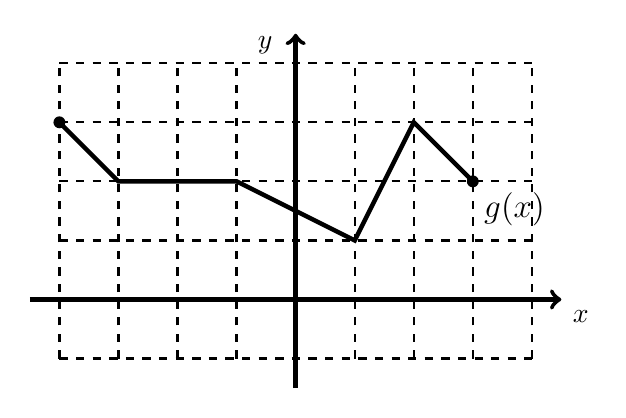
\begin{tikzpicture}[y=0.75cm, x=0.75cm,font=\sffamily]
        \begin{scope} %[shift={(0,8)}]
          %% ticks
          \draw[xstep = 1, ystep=1.0,black,dashed,thick] % very thin,opacity=0.85,
                 (-4.0,-1.0) grid ( 4.0, 4.0);
             %% axis
           \draw[ultra thick,->] (-4.5,0) -- coordinate (x axis mid) (4.5,0)
                node[anchor = north west] {$x$}; 
           \draw[ultra thick,->] (0,-1.5) -- coordinate (y axis mid) (0,4.5) 
                node[anchor = east,shift={(-0.2,-0.2)}]  {$y$};
            %% \draw[ultra thick,black] 
           \draw[ultra thick] plot coordinates
               {(-4,3) (-3,2) (-1,2) (1,1) (2,3) (3,2) }
               node[anchor=north west] {\large $g(x)$};
           \fill[black] (-4,3) circle [radius=0.5ex];
           %\fill[black] (-3,2) circle [radius=0.3ex];
           %\fill[black] (-1,2) circle [radius=0.3ex];
           %\fill[black] ( 1,1) circle [radius=0.3ex];
           %\fill[black] ( 2,3) circle [radius=0.3ex];
           \fill[black] ( 3,2) circle [radius=0.5ex];

           %\foreach \y in {-1,1,...,4} {
           %   \draw (1pt, \y) -- (-1pt, \y) node[yshift=-6,xshift=1,anchor=west] {$\y$};
           % }
           %\foreach \x in {-3,-2,-1,1,2,3} {
           %   \draw (\x,1pt) -- (\x,-1pt) node[yshift=-5,xshift=-1,anchor=east] {$\x$};
           % }

          \end{scope}
        \end{tikzpicture}
&
\begin{tabular}{l }
 $g(-4)$ \\ \\
 $g(-2)$ \\ \\
 all $x$ such that $g(x)=3$ \\ \\
 all $x$ such that $g(x)<2$ \\[1.5in]
\end{tabular}
\end{tabular}





\noindent \begin{tabular}{| l | }
\hline The \emph{domain} is the collection of all the numbers that go \emph{into} the function. When no domain \hfill \\is specified, the domain is the collection of all the numbers that make sense when you plug \\ them into the function. \\ \hline
\end{tabular}\\[.3in]

\noindent \begin{tabular}{| l | }
\hline The \emph{range} is the collection of all the numbers that \emph{come out of} the function. 
\\ \hline
\end{tabular}\\[.3in]
\item Determine the domain and range of the function $g(x)$ in the previous example. Then determine intervals where $g(x)$ is increasing, decreasing, or constant.\\[1in]


\newpage

\item Determine the domain of each of the following functions. Give your answer in interval notation.

\vspace{-.1in}
$$g(x) = -x^3 + 7x^2 + 17 \quad \quad \quad \quad \quad \quad f(x)=\sqrt{4x+5} \quad \quad  \quad \quad h(x)=\dfrac{1}{x^2-14}$$
\vfill



\end{enumerate}

\noindent \textbf{Student Learning Outcomes Check}

\begin{enumerate}
\item Can you determine whether a relation is a function?
\item Are you able to recognize and apply function notation?
\item Can you determine function characteristics including domain, range, increasing, decreasing, and constant?
\end{enumerate}

\noindent \textbf{If any of your answers were no, please ask about these topics in class.}


